\chapter{Scan Konvertierung}
Scan Konvertierung = Rasterung. Bezeichnet den Vorgang vom Übersetzen von Linien \& Polygone in Pixel.
\section{Rasterung Linie}
Man nehme als erstes Beispiel eine einfache Linie. Mathematisch könnte man diese ja so beschreiben:
\begin{displaymath}
y(x)=mx+b
\end{displaymath}
Gerastert müsste diese dann so aussehen wie in Abbildung \ref{fig:gerasterte_linie}.
\begin{figure}[!ht]
	\centering
	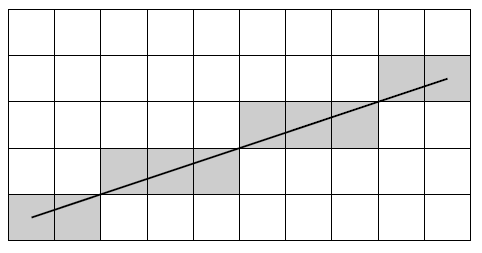
\includegraphics[width=0.4\linewidth]{fig/gerasterte_linie}
	\caption{Gerasterte Linie}
	\label{fig:gerasterte_linie}
\end{figure}
Pro Spalte haben wir ja immer nur 1 Pixel gesetzt hier, d.h wir müssen jeweils nur herausfinden, welche Zeile den geringsten Abstand zur korrekten Linie hat.



\subsection{Digital Differential Analyzer}
Beim Digital Differential Analyzer (DDA) berechnen wir zuerst den genauen Y-Wert, ganz nach der Formel \(y(x)=mx+b\). Dann runden wir dies auf die nächste ganze Zahl und haben den Wert, welcher Pixel gezeichnet werden soll. Das machen wir für jede Spalte - ist also entsprechend aufwändig zu berechnen, da für jeden Pixel eine Multiplikation gemacht werden muss. Besser wäre es, ausgehend vom Startpixel zu rechnen - denn in der Formel erhöht sich x ja immer um 1, das heisst es wird einfach immer \(+ m\) ausgegeben. Wir haben dann also:
\begin{displaymath}
y_{i+i}=y_i+m
\end{displaymath}
Das Verfahren ist aber immer noch mühsam, weil hier mit Gleitkommazahlen gerechnet wird und diese dann erst noch gerundet werden! Für Performancefreaks in der Computergrafik ein Graus.

\subsection{Mittelpunktschema - Linie}
Eine Linie kann ja eigentlich auch als folgende Gleichung dargestellt werden:
\begin{displaymath}
F(x,y) = ax+by+c = 0
\end{displaymath}
Die Distanz von einem Punkt \((x,y)\) zu dieser Linie wäre dann: (MEP?)
\begin{displaymath}
d = \frac{|ax+by+c|}{\sqrt{a^2+b^2}}
\end{displaymath}
Das heisst für alle x,y Werte ergibt die Gleichung 0 wenn sie auf der Linie sind - klar.\\Nehmen wir jetzt zusätzlich noch an, dass die Linie steigt, und zwar nicht stärker als 1. Wenn wir wieder Spalte für Spalte anschauen, kann es also nur sein, dass der nächste gezeichnete Pixel der direkt rechts vom jetzigen ist, oder dann der rechts schräg oben. Um dann zu entscheiden, welcher Punkt jetzt gezeichnet wird, setzen wir einen Punkt zwischen die beiden möglichen Pixel und setzen den in die Gleichung ein. Wenn diese etwas positives zurückliefert, dann ist die Linie oberhalb des Mittelpunktes und wir setzen den Pixel oben rechts. Ansonsten setzen wir ihn einfach rechts. In der Beispielgrafik \ref{fig:mittelpunktschema} bedeutet \textit{E} east, also rechts und \textit{NE} north east - oben rechts.
\begin{figure}[!ht]
	\centering
	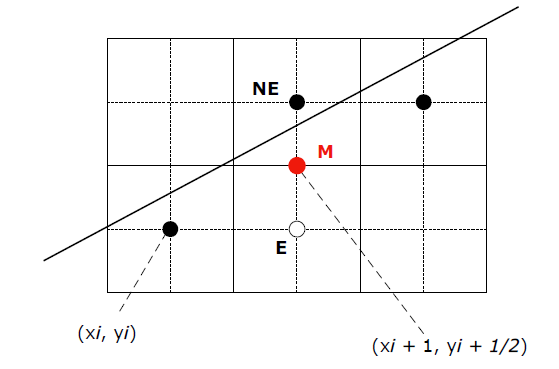
\includegraphics[width=0.4\linewidth]{fig/mittelpunktschema}
	\caption{Mittelpunktschema Grafik}
	\label{fig:mittelpunktschema}
\end{figure}\\
Wenn man es implementiert, hat man üblicherweise 2 Punkte - also \((x_0,y_0)\) und \((x_1,y_1)\). Dann gilt es nur noch, diese Werte in den untenstehenden Algorithmus einzufügen und los gehts.
\begin{figure}[!ht]
	\centering
	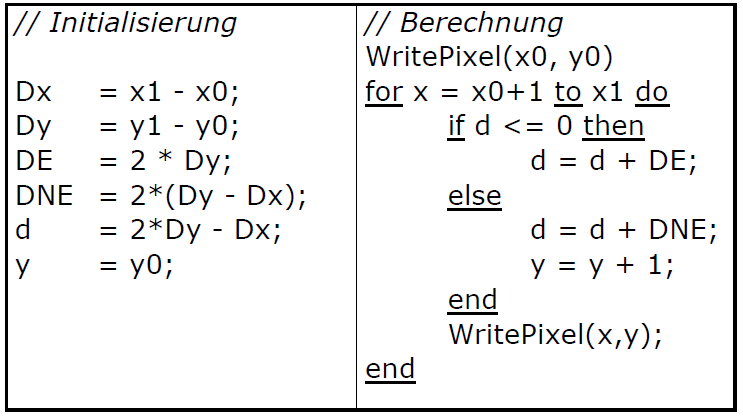
\includegraphics[width=0.4\linewidth]{fig/mittelpunktschema_algo}
	\caption{Mittelpunktschema Algorithmus}
	\label{fig:mittelpunktschema_algo}
\end{figure}
\section{Mittelpunktschema - Kreise}
Dasselbe wie für Linien. Zudem können wir sagen, wenn wir ja \((x,y)\) berechnet haben, haben wir auch \((x,-y)\),\((-x,y)\),\((-x,-y)\), \((y,x)\), \((-y,x)\), \((y,-x)\) und \((-y,-x)\) - also alle möglichen Kombinationen von +, -, x und y. Die mathematisch korrekte Formel für die Kreise wäre (r = Radius):
\begin{displaymath}
F(x,x) = x^2 + y^2 - r^2
\end{displaymath}
Der Punkt \((x_i,y_i)\) liegt gerade im zweiten Quadranten. Das heisst der Kreis sieht zur Zeit so aus, wie in Abbildung \ref{fig:mittelpunktschema_kreis}. Das heisst wir sind wie bei der Linie beim Punkt \((x_i,y_i)\) und müssen jetzt entscheiden, zeichnen wir den nächsten Pixel rechts von uns (east - \textit{E}), oder halt rechts unten (south east - \textit{SE}). Die Distanz \textit{d} berechnet sich hier so, also eigentlich einfach die normale Kreisformel, wo einfach noch ein \(+1\) eingesetzt wurde beim x - Wert und beim y - Wert ein \(- \frac{1}{2}\), da der Kreis ja etwas fällt.
\begin{displaymath}
d = (x_i + 1)^2 + (y_i - \frac{1}{2})^2 - r^2
\end{displaymath}
\begin{figure}[!ht]
	\centering
	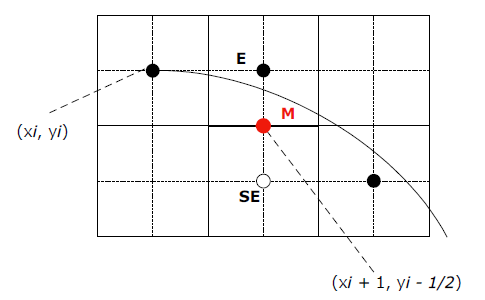
\includegraphics[width=0.4\linewidth]{fig/mittelpunktschema_kreis}
	\caption{Mittelpunktschema Grafik für den Kreis}
	\label{fig:mittelpunktschema_kreis}
\end{figure}

\begin{figure}[!ht]
	\centering
	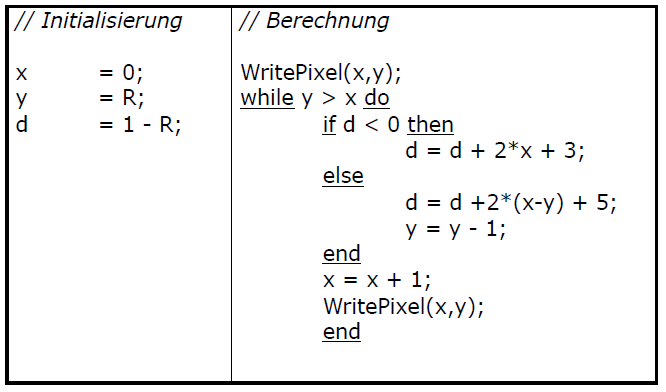
\includegraphics[width=0.4\linewidth]{fig/mittelpunktschema_algo_kreis}
	\caption{Mittelpunktschema Algorithmus für den Kreis}
	\label{mittelpunktschema_algo_kreis}
\end{figure}
\section{Füllen von Flächen mit Farbe}
Sehr easy. Einfach dieser rekursive Algorithmus.
\begin{figure}[!ht]
	\centering
	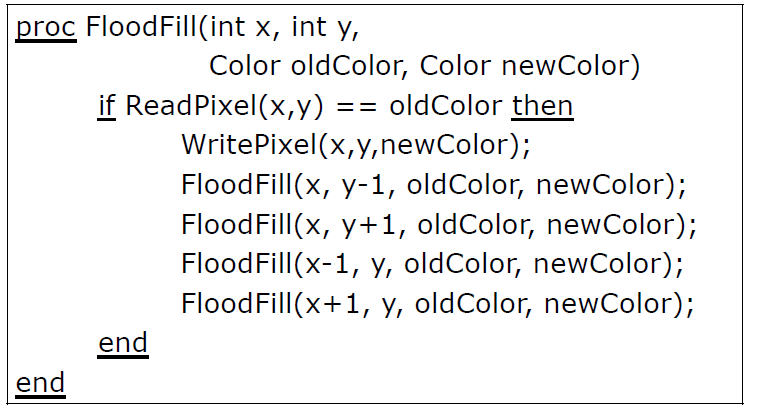
\includegraphics[width=0.4\linewidth]{fig/flaeche_fill}
	\caption{Füll Algorithmus}
	\label{flaeche_fill}
\end{figure}
Wenn man innehralb einer Berandung das macht, dann einfach \texttt{ReadPixel(x,y) != boundaryColor}.

\section{Füllen von Polygonen}
Hier verwendet man den Scanlinien Algorithmus. Das heisst, wir gehen wie bei einem alten Röhrenfernseher von oben nach unten und zeichnen Zeilenweise die Pixel ins Polygon, siehe Abbildung \ref{scanlinie}. 
\begin{figure}[!ht]
	\centering
	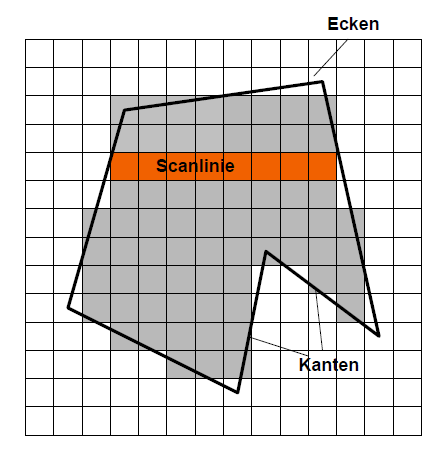
\includegraphics[width=0.4\linewidth]{fig/scanlinie}
	\caption{Scanlinien Algorithmus Grafik}
	\label{scanlinie}
\end{figure}
Damit wir wissen, von wo nach wo die Pixel gezeichnet werden sollen, müssen wir ja die Schnittpunkte der Kanten berechnen, welche die aktuelle Scanlinie schneiden. Damit das effizient geschieht, sind sie bereits vorsortiert in Kantentabellen:
\begin{enumerate}
	\item \textbf{Kantentabelle \textit{edgetable}}\\
	Alle Kanten des Polygons sind nach minimaler y Koordinate \(y_{min}\) sortiert. Wenn zwei Kanten denselben \(y_{min}\) haben, werden sie nach x sortiert.
	\item \textbf{Aktive Kanten (\textit{AET})}\\
	Hier werden alle Kanten gespeichert, die von der aktuellen Scanlinie geschnitten werden, dies sortiert nach x.
\end{enumerate}
\begin{figure}[!ht]
	\centering
	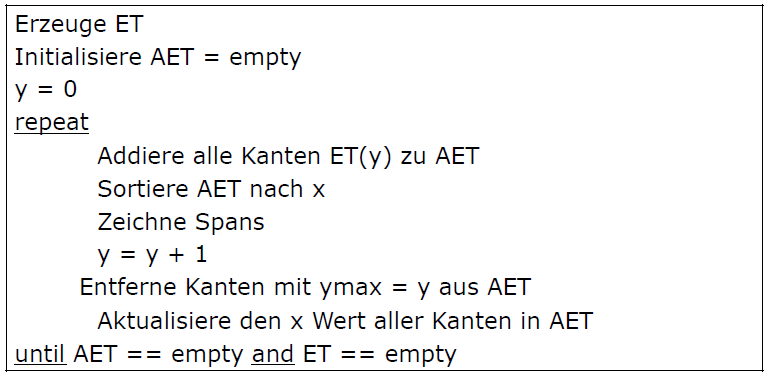
\includegraphics[width=0.5\linewidth]{fig/scanlinie_algo}
	\caption{Scanlinien Algorithmus}
	\label{scanlinie_algo}
\end{figure}
\begin{figure}
\centering
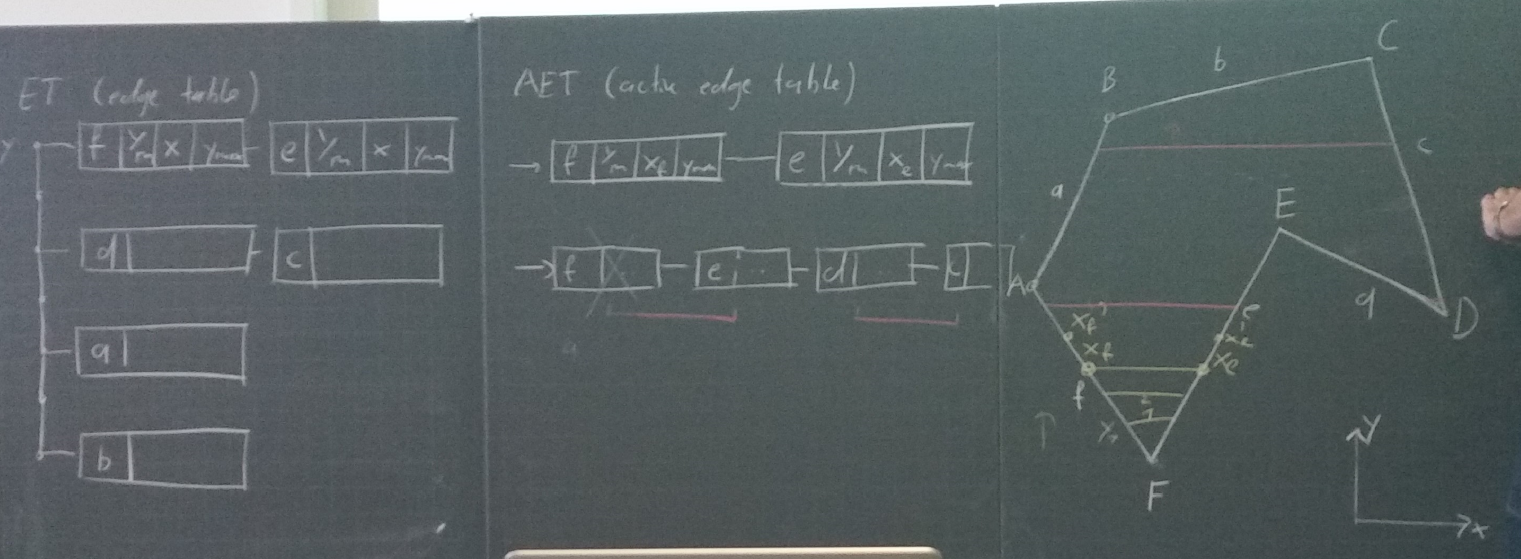
\includegraphics[width=0.7\linewidth]{fig/scanlinie_tafel}
\caption{Scanlinien Algorithmus}
\label{fig:scanlinie_tafel}
\end{figure}

\section{Dreiecke zeichnen - à la Brute Force}
Das ist furzeinfach. Wir haben oben ja gesehen, dass wir mit der Liniengleichung bestimmen können, ob ein Punkt oberhalb oder unterhalb einer Linie ist. Ein Dreieck besteht ja eigentlich nur aus 3 Linien, das heisst wir prüfen für jeden Pixel, ob die Gleichung für alle Dreieckslinien aufgeht - wenn ja zeichnen wir ihn, sonst lassen wirs sein. Die in Abbildung \ref{dreiecke_zeichnen} eingefärbten Regionen bezeichnen die Region, welche \textit{innerhalb} der Kante des Dreiecks liegen. Dort, wo sich alle Farben überlappen, dort werden die Pixel entsprechend gezeichnet.
\begin{figure}[!ht]
	\centering
	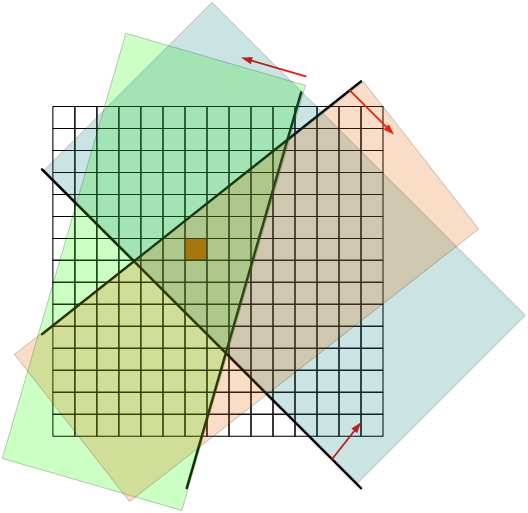
\includegraphics[width=0.5\linewidth]{fig/dreiecke_zeichnen}
	\caption{Dreiecke Zeichnen Brute Force Algorithmus}
	\label{dreiecke_zeichnen}
\end{figure}
\section{Anti Aliasing}
Wir haben hier Linien gezeichnet, die allerdings einen extremen Treppeneffekt hätten, wenn wir sie 1:1 auf dem Monitor darstellen würden. Wir schauen kurz 2 Techniken an, die diesen Treppeneffekt minimieren.
\subsection{Prefiltering}
\begin{figure}[!ht]
	\centering
	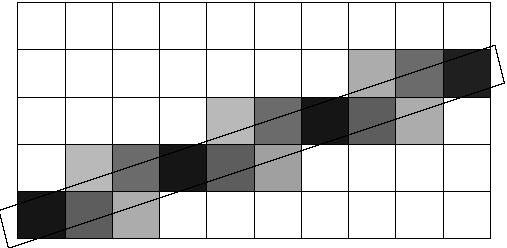
\includegraphics[width=0.5\linewidth]{fig/prefiltering}
	\caption{Prefiltering Algorithmus}
	\label{prefiltering}
\end{figure}
Hier berechnet man die Fläche der Linie auf dem Pixel und wählt proportional dazu die Intensität der Farbe. 
\subsection{Supersampling}
Das Prinzip von Supersampling ist, dass man viel mehr Pixel berechnet, als eigentlich nötig wären. Nehmen wir das 2x2 Super Sampling, wo wir 4x mehr Pixel generieren und diese dann zusammenrechnen, wie in Abbildungen \ref{supersampling_1}, \ref{supersampling_2} gezeigt.
\begin{figure}[!ht]
	\centering
	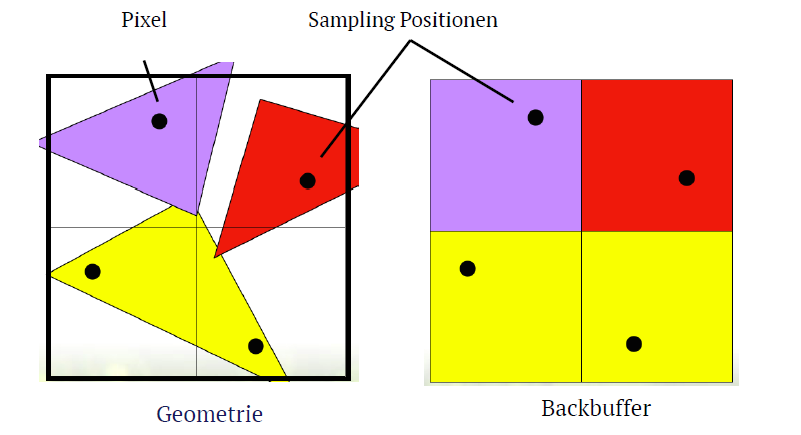
\includegraphics[width=0.5\linewidth]{fig/supersampling_1}
	\caption{Supersampling 1}
	\label{supersampling_1}
\end{figure}
\begin{figure}[!ht]
	\centering
	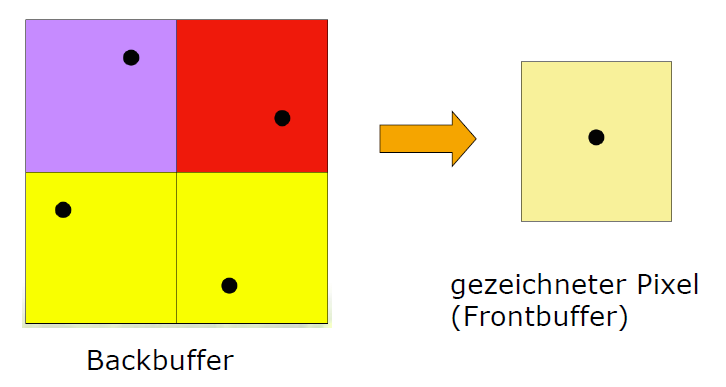
\includegraphics[width=0.5\linewidth]{fig/supersampling_2}
	\caption{Supersampling 2}
	\label{supersampling_2}
\end{figure}
Im Detail berechnen wir die Geometrie unserer Objekte und definieren sog. Sampling Positionen. Die Farbe an diesen sampling Positionen bestimmt dann die Farbe des ganzen Pixels - welcher im Backbuffer abgelegt wird und eben eine 4x höhere Auflösung hat als gezeigt. Die Farben des Backbuffers werden zum Schluss zusammengerechnet und es wird genau 1 Pixel gezeichnet, der Frontbuffer.